% Copyright 2022 by Sébastien Descotes-Genon
%
% This file may be distributed and/or modified
%
% 1. under the LaTeX Project Public License and/or
% 2. under the GNU Public License.
%


\documentclass{beamer}

\usepackage{array,amsmath}
\newcolumntype{L}{>$l<$}



% Setup appearance:

\usetheme{IJCLab}

\pgfdeclareimage[height=2cm]{LogoIJCLab}{example-fig/LogoIJCLab}
\pgfdeclareimage[height=1.3cm]{LogoCNRS}{example-fig/LogoCNRS}
\pgfdeclareimage[height=1cm]{LogoUPSay}{example-fig/LogoUPSay}


\usepackage[english]{babel}
\usepackage[T1]{fontenc}


\AtBeginSection[]
{
  \begin{frame}
    \frametitle{Table of Contents}
    \tableofcontents[currentsection]
  \end{frame}
}



% Author, Title, etc.

\title[FGCM Simulation]{\large Review of the Forward Global Photometric Calibrationn\\
{\small inspired from the DES article Burke et al. 2017}}

\titlegraphic{\begin{center}\qquad\pgfuseimage{LogoCNRS}\qquad\quad\qquad\quad\pgfuseimage{LogoIJCLab}\qquad\qquad\pgfuseimage{LogoUPSay}\end{center}}

\author[S. Dagoret-Campagne]{
Sylvie Dagoret-Campagne,Marc Moniez, Martin Rodriguez Monroy, Joseph Chevalier,}
\institute[IJCLab]{
  IJCLab,
  CNRS/IN2P3 \& Université Paris-Saclay,
  Orsay, France }
  
  % Caution  : This is not the affiliation to be used to sign articles. 
  % Please refer to the intranet : Bibliothèque/IST / Règles de publication
     
\date[IJCLab, Dec 16th 2022]{DESC PCWG, December 16th 2022}






% The main document with a few examples
%%%%%%%%%%%%%%%%%%%%%%%%%%%%%%%%%%%%%%%%%%%%%%%%%%%%%%%%%%%%%%%%%%%%%%%%%%%%%%
\begin{document}

%==================================================================================================================================
\begin{frame}
  \titlepage
\end{frame}
%==================================================================================================================================



%==================================================================================================================================
%\begin{frame}{Outline}
%  \tableofcontents
%\end{frame}
%==================================================================================================================================


% see example https://tex.stackexchange.com/questions/62902/text-column-in-array
% Define a text column environnement
%\usepackage{array,amsmath}
%\newcolumntype{L}{>$l<$}

%\begin{frame}
%\begin{equation*}
%    \begin{array}{L@{\quad}c@{{}={}}c}
%       some text:            & x^2 & x^2 \\
%       more thoughts:        & y^2 & y^2 \\
%       really deep thoughts: & z^2 & z^2
%    \end{array}
%\end{equation*}
%\end{frame}

%=================================================================================================================================
%\begin{frame}{Magnitude calibration of astronomical objects}
%\begin{alertblock}{Article Burke et al. 2017, Formula (16) }
%\begin{equation*}
%    \begin{array}{l@{{}{}}c c@{\quad}L}
%               m_b^{std} =   & -2.5 \log_{10}(ADU_b^{obs}) & \longrightarrow  & ADU photometric counts     \\
%                & +  2.5 \log_{10}\left(\mathbb{I}_0^{obs}(b)\right)  &\longrightarrow  &  {\color{red}0th order transmission term} \\
%                 & + ZPT^{AB}_{obs}  & \longrightarrow & Zero Point magnitude \\
%                 &  +  2.5 \log_{10} 
%	\left( 
%	\frac{\int_0^\infty F_\nu(\lambda) \times \phi_b^{obs}(\lambda) d\lambda }{\int_0^\infty F_\nu(\lambda) \times \phi_b^{std}(\lambda) d\lambda} 
%	\right) & \longrightarrow & {\color{blue}SED Color correction term}
%    \end{array}
%\end{equation*}
%\end{alertblock}
%{\footnotesize
%\begin{block}{Calibration quantities for each observation:}
%\begin{equation*}
%\begin{array}{L@{\quad}ccc}
%transmission integral : & \mathbb{I}_0^{obs}(b) & \equiv & \int_0^\infty S^{obs}_b(\lambda) \frac{d\lambda}{\lambda} \\
%zero point link to AB-flux unit/CCD : & ZPT^{AB}_{obs} & \equiv & 2.5 \log_{10} \left( \frac{A \Delta T F^{AB}}{gh}\right)
%\end{array} 
%\end{equation*}
%\end{block}
%\begin{itemize}
%\item Total observation transmission : $S_b^{obs}(\lambda) = S^{atm}(\lambda) \times S_b^{inst}(\lambda)$
%\item Normalized passband : $\phi_b^{obs} (\lambda,t) = \frac{S_b^{obs}(\lambda,t)\frac{1}{\lambda}}{\int_0^\infty S^{obs}_b(\lambda,t) \frac{d\lambda}{\lambda}}$
%\end{itemize}
%}
%\end{frame}
%=================================================================================================================================



%%%%%%%%%%%%%%%%%%%%%%%%%%%%%%%%%%%%%%%%%%%%%%%%%%%%%%%%%%%%%%%%%%%%%%%%%%%%%%%%%%%%%%%%%
\section{Photometric correction for standard magnitude}
\begin{frame}\sectionpage\end{frame}
%%%%%%%%%%%%%%%%%%%%%%%%%%%%%%%%%%%%%%%%%%%%%%%%%%%%%%%%%%%%%%%%%%%%%%%%%%%%%%%%%%%%%%%%%


%=================================================================================================================================
\begin{frame}{Standard magnitude calibration of objects}
\begin{alertblock}{Article Burke et al. 2017, Formula (16)}
\begin{equation*}
    \begin{array}{l@{{}{}}c c@{\quad}L}
               m_b^{std} =   & -2.5 \log_{10}(ADU_b^{obs}) & \longrightarrow  & ADU photometric counts     \\
                & +  2.5 \log_{10}\left(\frac{\mathbb{I}_0^{obs}(b)}{\mathbb{I}_0^{std}(b)}\right)  &\longrightarrow  &  {\color{red}0th order transmission term} \\
                 & + ZPT^{AB}_{obs} + 2.5 \log_{10}\left(\mathbb{I}_0^{std}(b)\right) & \longrightarrow & Zero Point magnitude \\
                 &  +  2.5 \log_{10} 
	\left( 
	\frac{\int_0^\infty F_\nu(\lambda) \times \phi_b^{obs}(\lambda) d\lambda }{\int_0^\infty F_\nu(\lambda) \times \phi_b^{std}(\lambda) d\lambda} 
	\right) & \longrightarrow & {\color{blue}SED Color correction term}
    \end{array}
\end{equation*}
\end{alertblock}
{\footnotesize
\begin{block}{Calibration quantities for each observation:}
\begin{equation*}
\begin{array}{L@{\quad}ccc}
transmission integral : & \mathbb{I}_0^{obs}(b) & \equiv & \int_0^\infty S^{obs}_b(\lambda) \frac{d\lambda}{\lambda} \\
zero point link to AB-flux unit/CCD : & ZPT^{AB}_{obs} & \equiv & 2.5 \log_{10} \left( \frac{A \Delta T F^{AB}}{gh}\right)
\end{array} 
\end{equation*}
\end{block}
\begin{itemize}
\item Total transmission : $S_b^{obs}(\lambda) = S^{atm-obs}(\lambda) \times S_b^{inst-obs}(\lambda)$
\item Normalized passband : $\phi_b^{c=obs,std} (\lambda,t) = \frac{S_b^{c}(\lambda,t)\frac{1}{\lambda}}{\int_0^\infty S^{c}_b(\lambda,t) \frac{d\lambda}{\lambda}}$
\end{itemize}
}
\end{frame}
%========================================================================================================================




% Slide 2
%=================================================================================================================================
\begin{frame}{Interpretation of correction terms to $m_{std}$}
{\footnotesize
The standard transmission is chosen apriory thus $\mathbb{I}_0^{std}(b)$ is calculated
}
{\footnotesize
\begin{tabular}{llll} \hline
a)&0th order corr term : & relative attenuation in $b$ & $2.5 \log_{10}\left(\frac{\mathbb{I}_0^{obs}(b)}{\mathbb{I}_0^{std}(b)}\right)$ \\
b)&1st order corr term : & SED color correction& $ 2.5 \log_{10} 
	\left( 
	\frac{\int_0^\infty F_\nu(\lambda) \times \phi_b^{obs}(\lambda) d\lambda }{\int_0^\infty F_\nu(\lambda) \times \phi_b^{std}(\lambda) d\lambda} 
	\right)$ \\
c)&constant term/CCD/exp: & Zero point to measure & $ZPT^{AB}_{obs}\equiv  2.5 \log_{10} \left( \frac{A \Delta T F^{AB}}{g_{el}h}\right)$ \\
d)&constant term/band : & Calculated & $2.5 \log_{10}\left(\mathbb{I}_0^{std}(b)\right)$ \\  \hline
\end{tabular}


\begin{itemize}
\item a) requires atmospheric transparency either by direct measurement with Auxtel or indirectly by fitting air-transparency in LSST-FGCM atmospheric model or combining both,
\item b) requires atmospheric transparency as well:
\begin{itemize}
\item stars : requires the magnitude color type of the stars 
\item galaxies and other : requires to classify by colors (by example for PhotoZ
\end{itemize}
\item c) Set the flux scale unit per CCD per exposure and is band independent.
\begin{itemize}
\item absorbs grey component common to all bands, (ex clouds, ageing,...)
\item measured with the contraints provided by the calibration star in the Monster Catalog
\end{itemize}
\end{itemize}
}

\end{frame}
%========================================================================================================================


%%%%%%%%%%%%%%%%%%%%%%%%%%%%%%%%%%%%%%%%%%%%%%%%%%%%%%%%%%%%%%%%%%%%%%%%%%%%%%%%%%%%%%%%%
\section{Order 0 band correction term}
\begin{frame}\sectionpage\end{frame}
%%%%%%%%%%%%%%%%%%%%%%%%%%%%%%%%%%%%%%%%%%%%%%%%%%%%%%%%%%%%%%%%%%%%%%%%%%%%%%%%%%%%%%%%%



%========================================================================================================================
\begin{frame}{Relative ratio of integrals}
Focusing on atmosphere component variations defined as
$\theta^{atm}= PWV, O_3, aerosols$
\begin{alertblock}{}
\begin{equation*}
\left(\frac{\mathbb{I}_0^{obs}(b,z_{obs},\theta_{obs}^{atm})}{\mathbb{I}_0^{std}(b,z_{std},\theta_{std}^{atm})}\right) =
\underbrace{\left(\frac{\mathbb{I}_0^{obs}(b,z_{obs},\theta_{obs}^{atm})}{\mathbb{I}_0^{std}(b,z_{obs},\theta_{std}^{atm})}\right)}_{1:ratio\;at \; same \; z_{obs}\; \& \; \neq \; \theta^{atm}} \times \underbrace{\left(\frac{\mathbb{I}_0^{std}(b,z_{obs},\theta_{std}^{atm})}{\mathbb{I}_0^{std}(b,z_{std},\theta_{std}^{atm})}\right)}_{2:calculable \; ratio \;at \; z_{obs}\neq z_{std} }
\end{equation*}
\end{alertblock}
\begin{itemize}
\item 1 : $\left(\frac{\mathbb{I}_0^{obs}(b,z_{obs},\theta_{obs}^{atm})}{\mathbb{I}_0^{std}(b,z_{obs},\theta_{std}^{atm})}\right)$ : numerator obtained by the {\bf measurement of atmospheric transmission for each exposure}, denominator calculated at observation $z_{obs}$ (small corrections at ~10 mmag level),
\item 2 : $\left(\frac{\mathbb{I}_0^{std}(b,z_{obs},\theta_{std}^{atm})}{\mathbb{I}_0^{std}(b,z_{std},\theta_{std}^{atm})}\right)$ : calculable ratio assuming knowledge of atmospheric model (large corrections at ~100 mmag level). 
\end{itemize}


\end{frame}
%========================================================================================================================




%========================================================================================================================
%\begin{frame}{Order 0 magnitude corrections at different airmass}
%\begin{itemize}
%\item standard transmission, standard atmosphere at airmass $z=z_{std}$
%\item observed transmission, standard atmosphere at airmass $z_{obs} \ne z_{std}$
%\end{itemize}

%\begin{columns}
%\begin{column}{0.6\textwidth}
%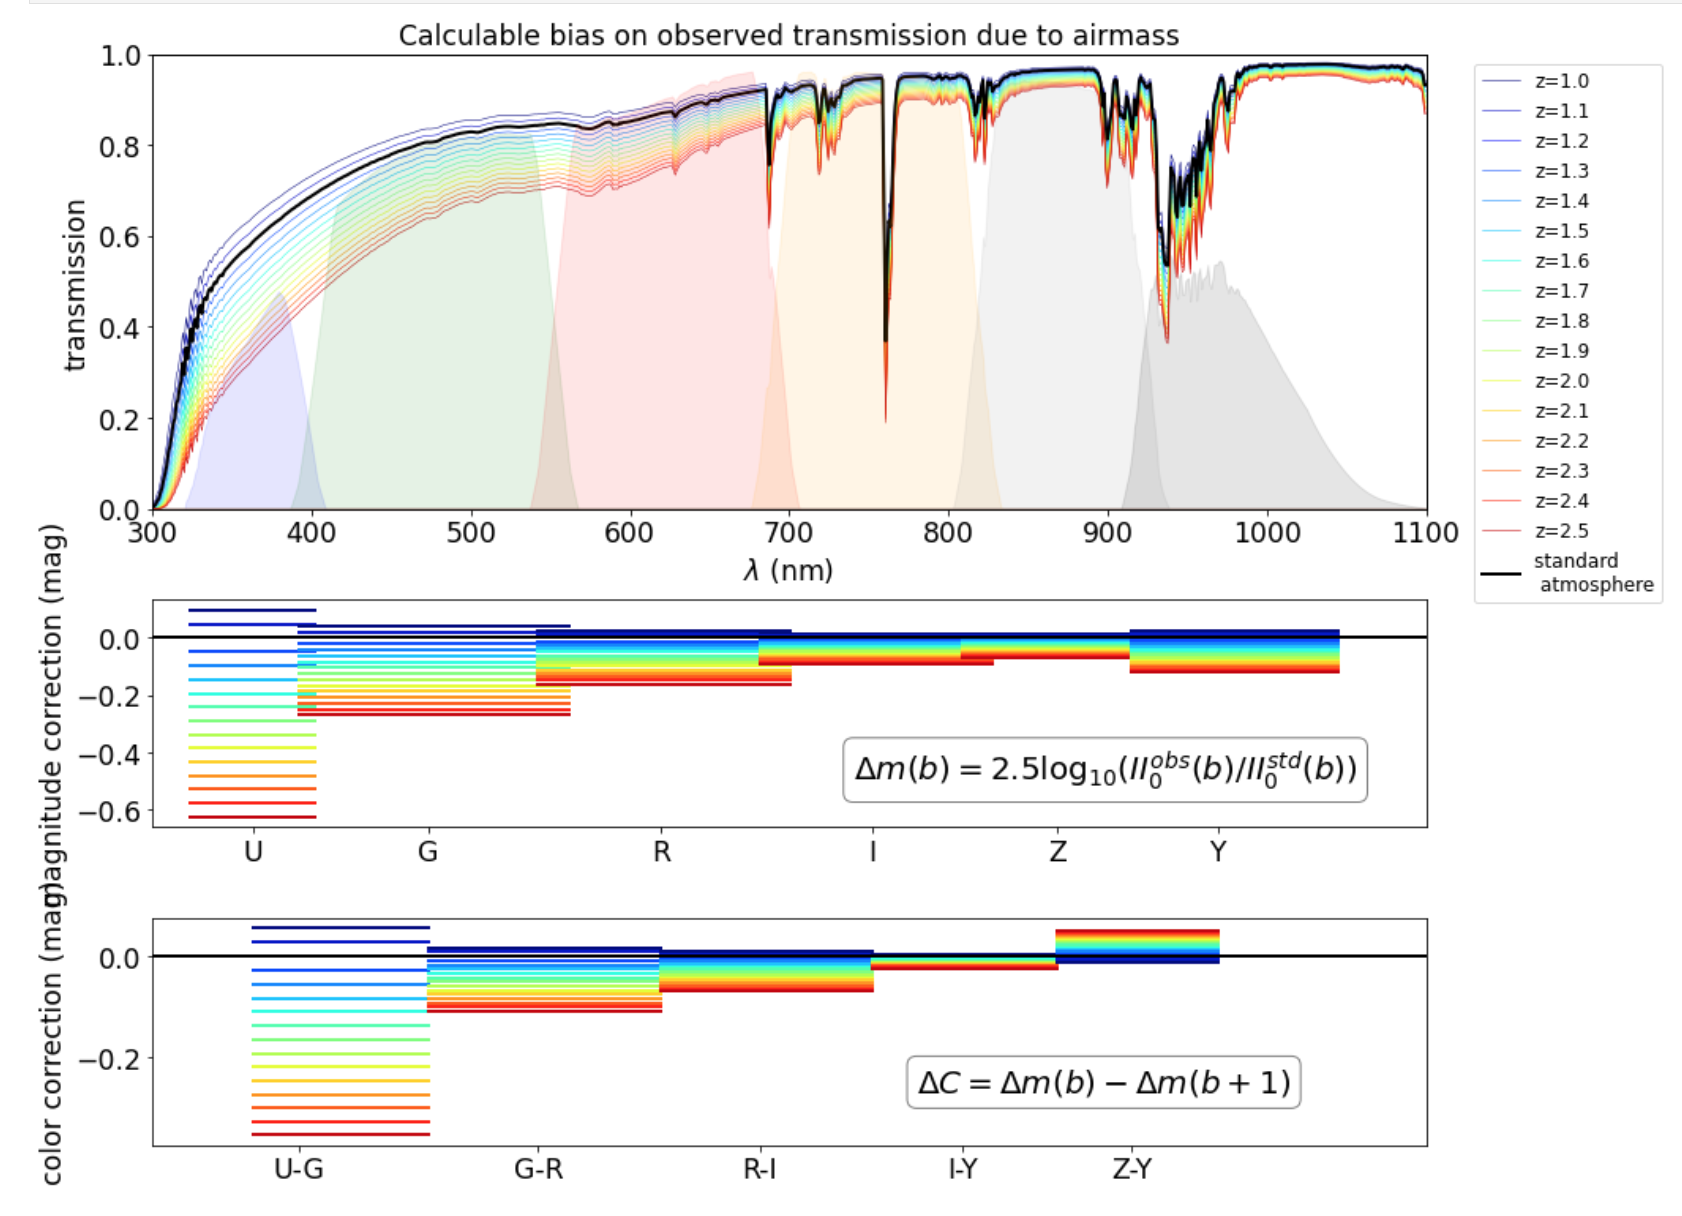
\includegraphics[width=8cm,angle=0]{figs/PCCorr/fig1_PCCorrOrder0th_airmass.png}
%\end{column}
%\begin{column}{0.4\textwidth}  %%<--- here
%\centering
%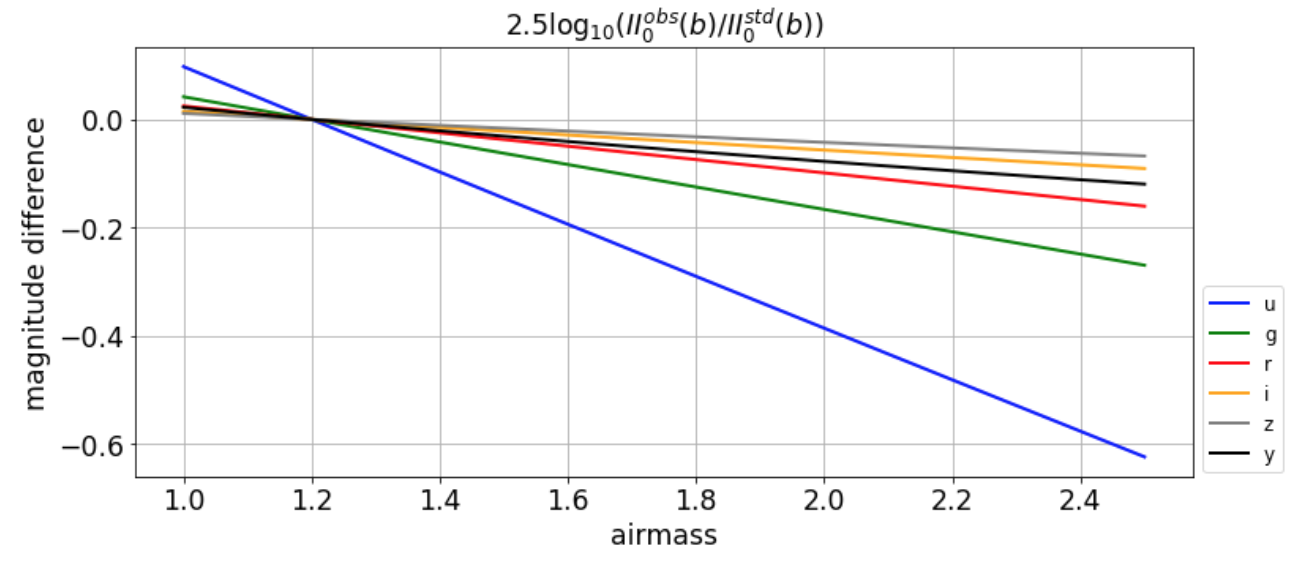
\includegraphics[width=4cm,angle=0]{figs/PCCorr/fig2_PCCorrOrder0th_airmass.png}
%\end{column}
%\end{columns}  
%\end{frame}
%========================================================================================================================

%========================================================================================================================
\begin{frame}{Order corrections at different airmass}

\begin{tabular}{cc}
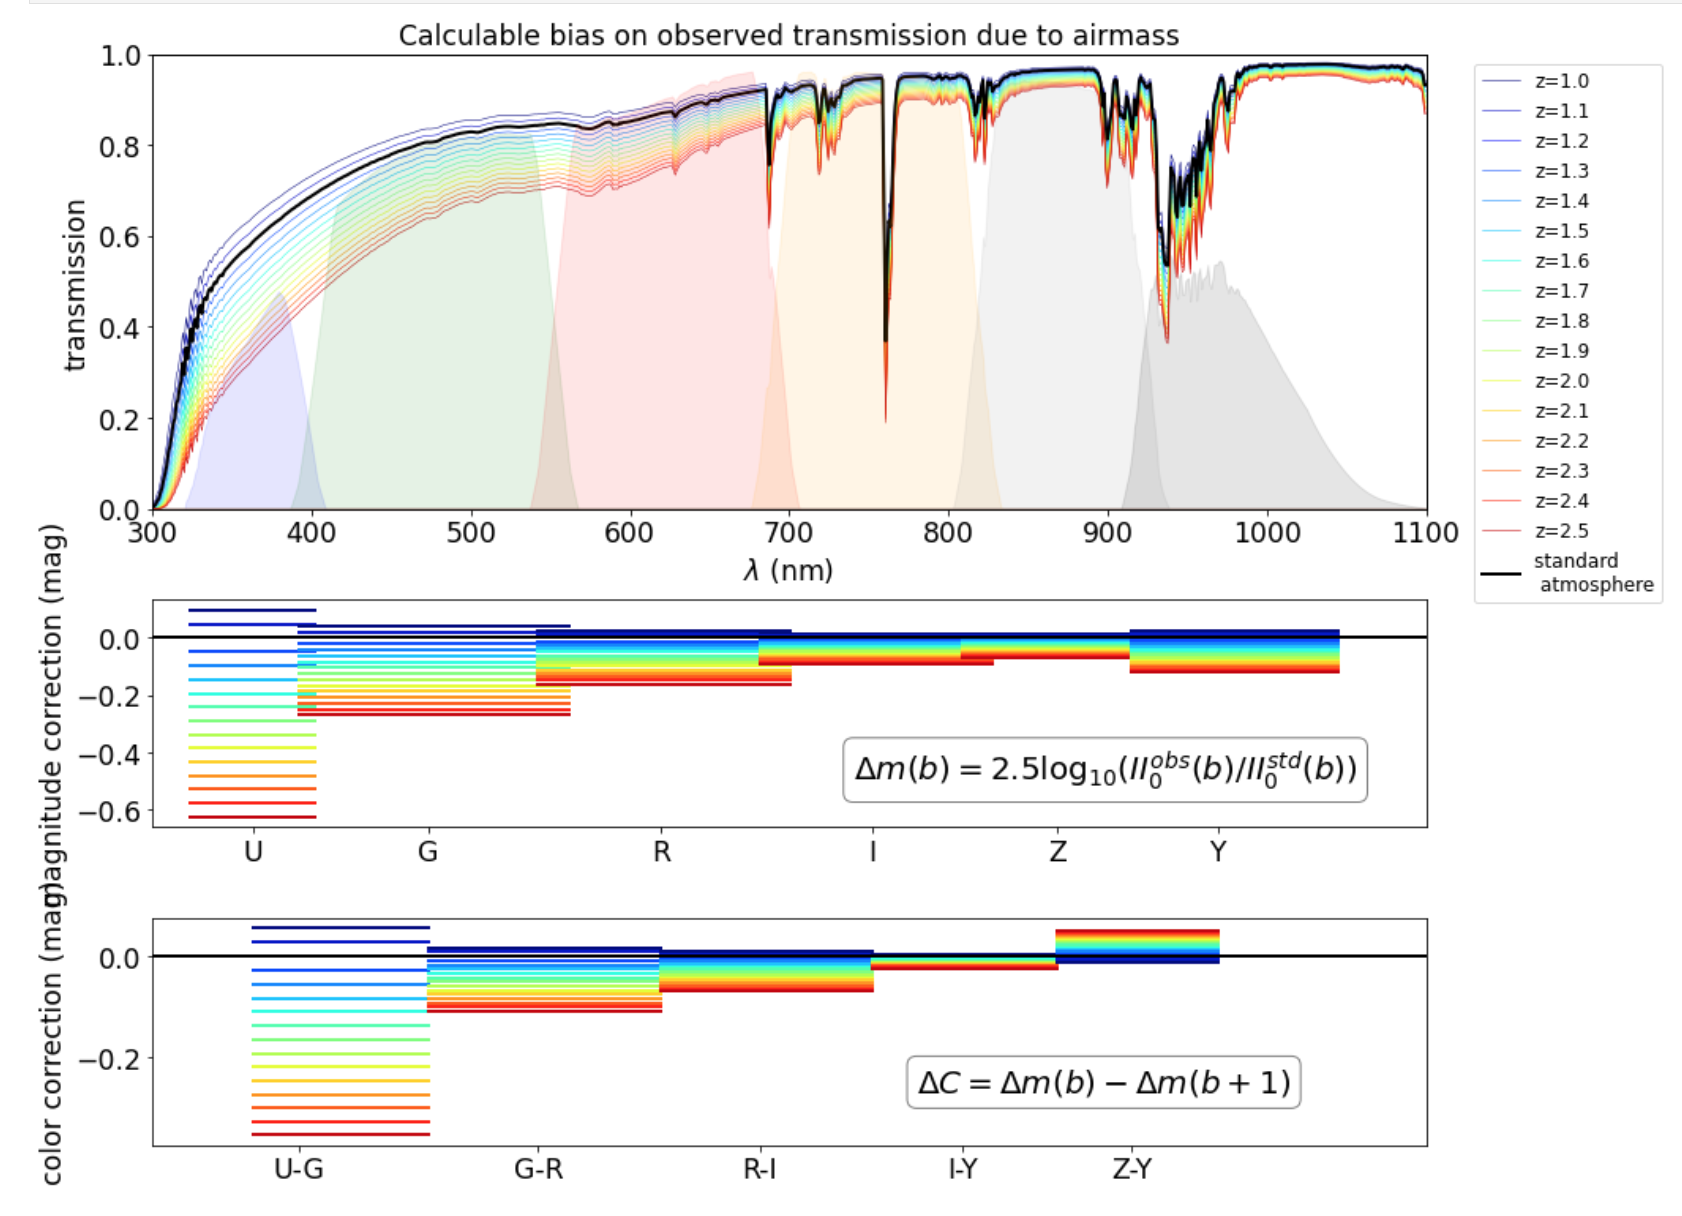
\includegraphics[width=6cm,height=6.5cm,angle=0]{figs/PCCorr/fig1_PCCorrOrder0th_airmass.png} &
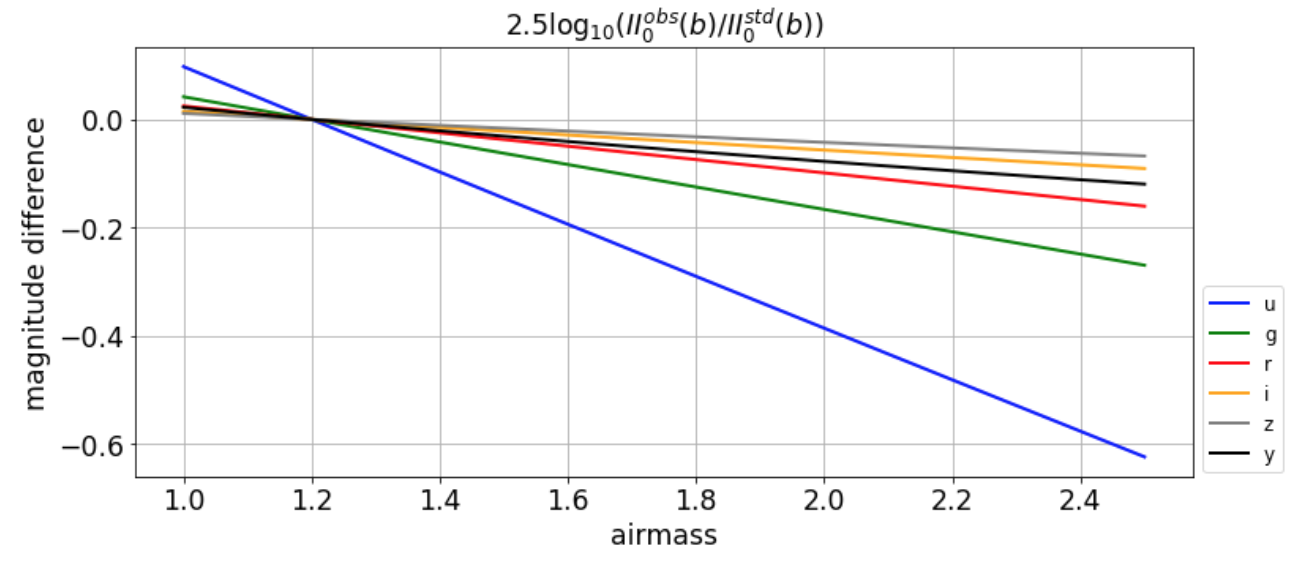
\includegraphics[width=5.5cm,height=4cm,angle=0]{figs/PCCorr/fig2_PCCorrOrder0th_airmass.png}
\end{tabular}
\end{frame}
%========================================================================================================================

%========================================================================================================================
\begin{frame}{Order corrections at different PWV}

\begin{tabular}{cc}
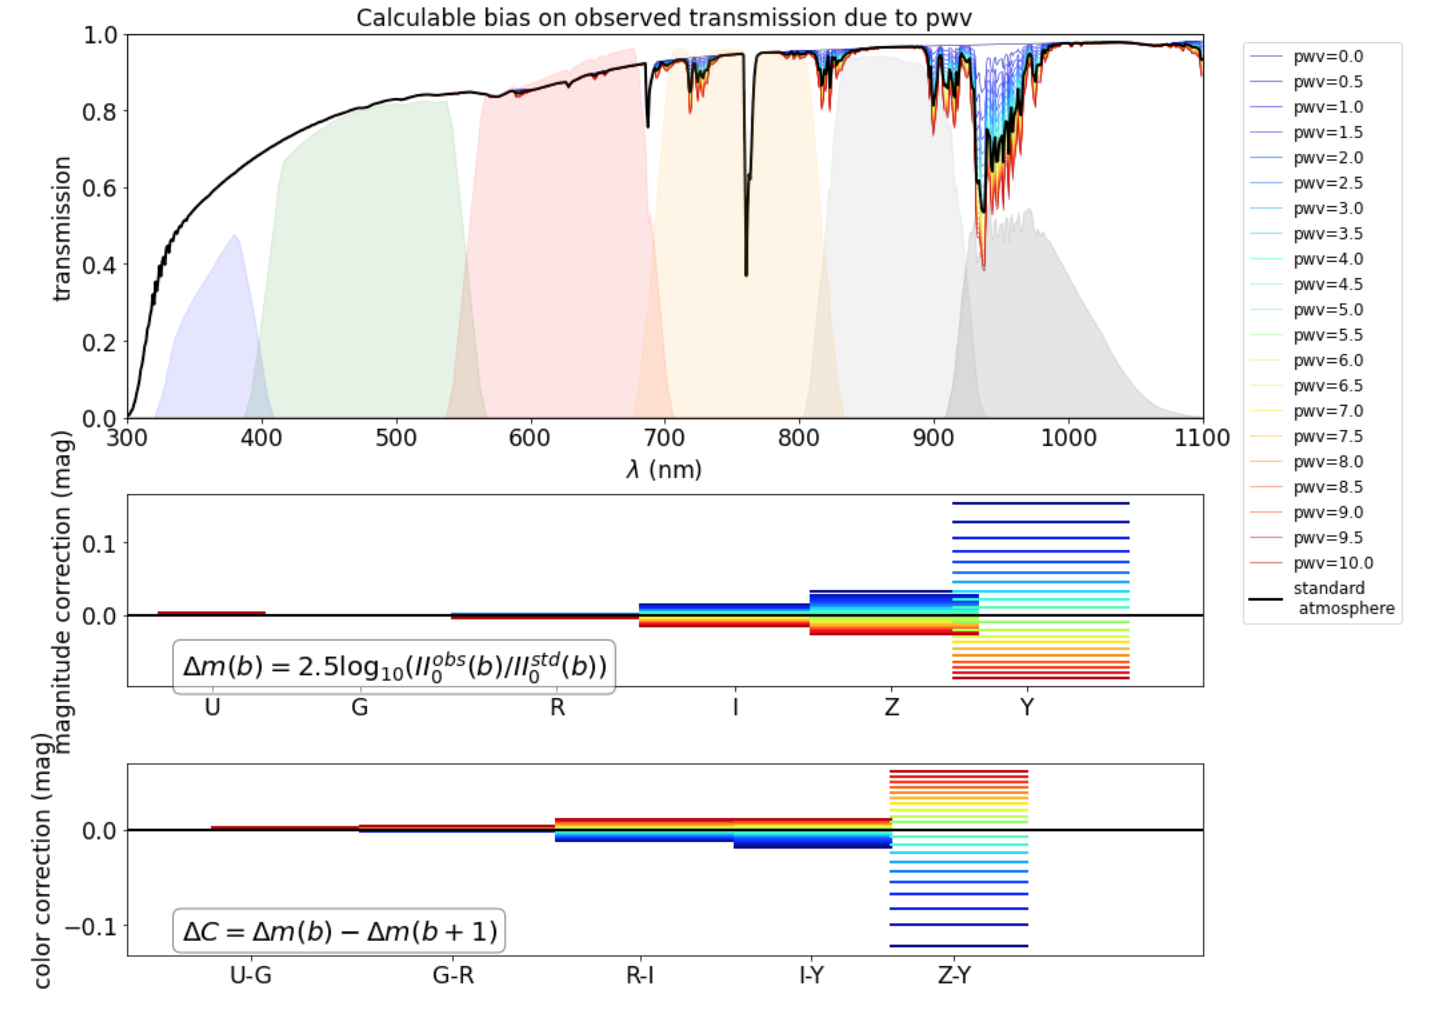
\includegraphics[width=6cm,height=6.5cm,angle=0]{figs/PCCorr/fig1_PCCorrOrder0th_PWV.png} &
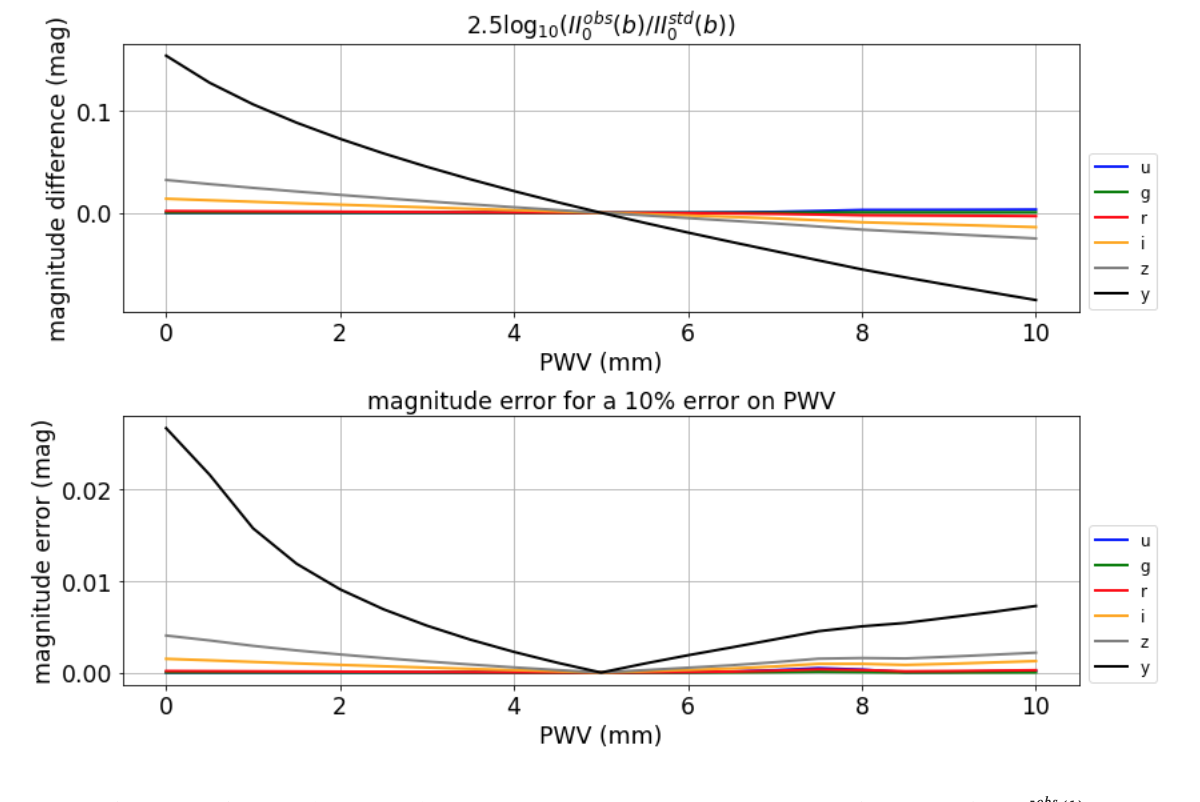
\includegraphics[width=5.5cm,height=6cm,angle=0]{figs/PCCorr/fig2_PCCorrOrder0th_PWV.png}
\end{tabular}
\end{frame}
%========================================================================================================================


%========================================================================================================================
\begin{frame}{Order corrections at different VAOD}

\begin{tabular}{cc}
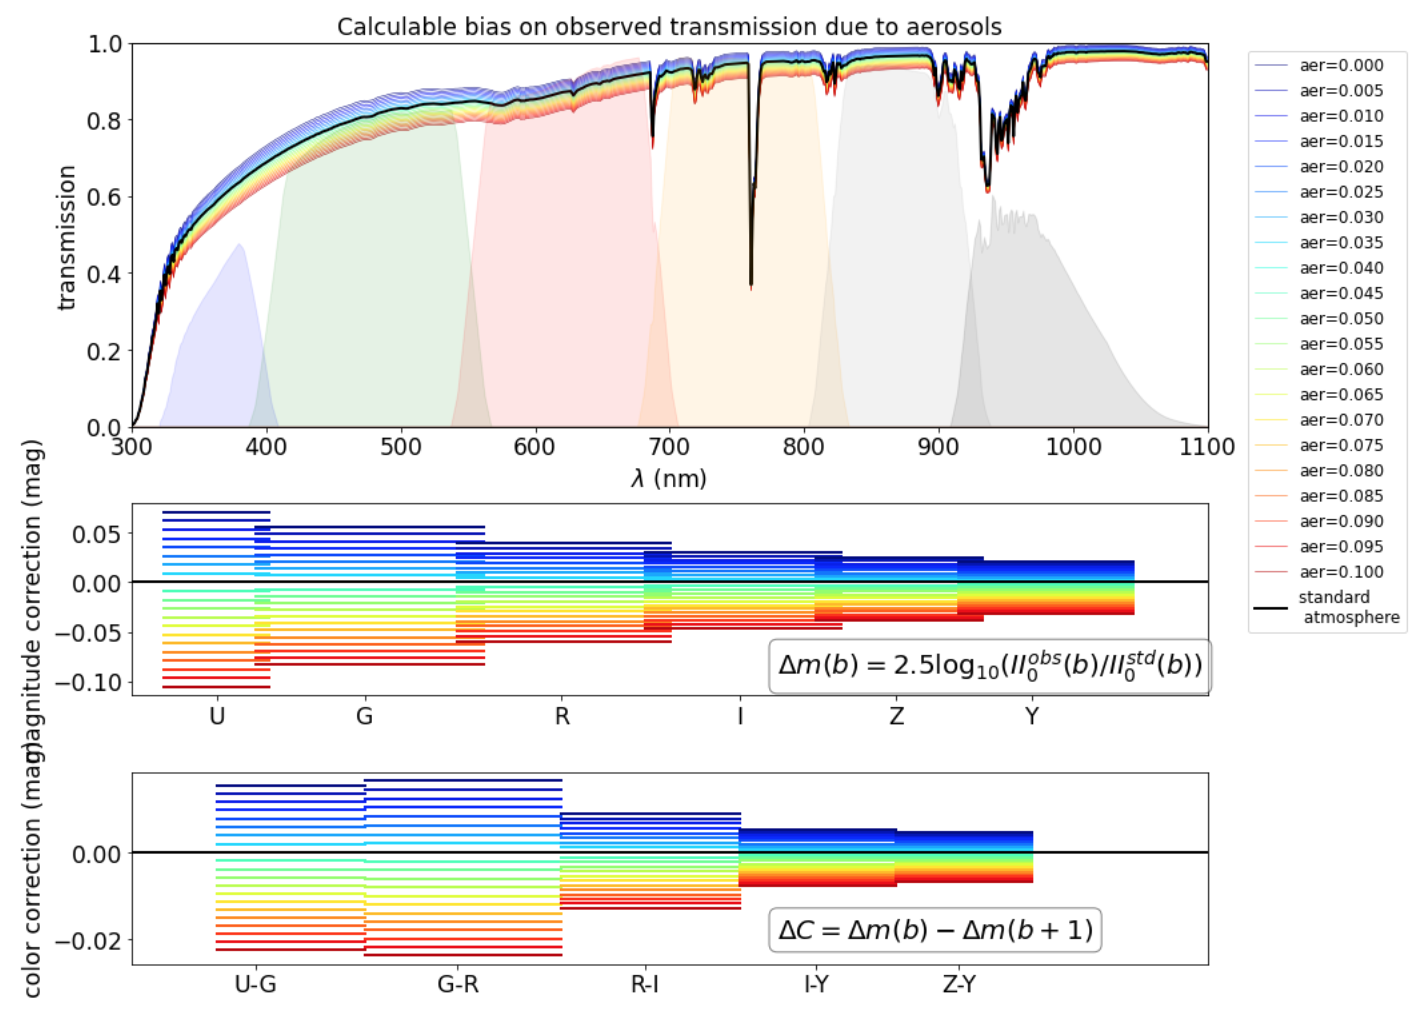
\includegraphics[width=6cm,height=6.5cm,angle=0]{figs/PCCorr/fig1_PCCorrOrder0th_aer.png} &
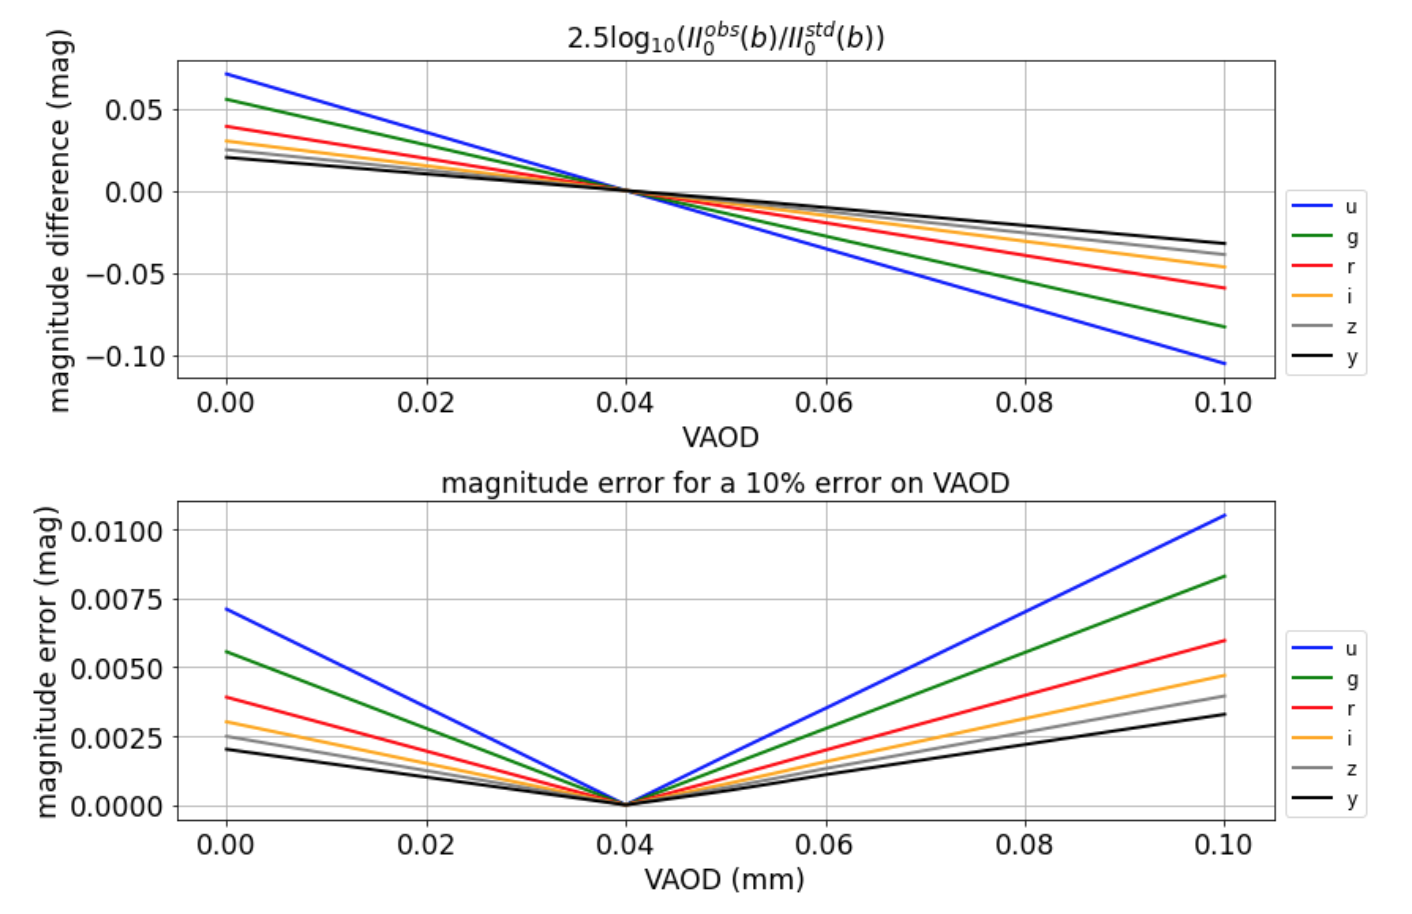
\includegraphics[width=5.5cm,height=6cm,angle=0]{figs/PCCorr/fig2_PCCorrOrder0th_aer.png}
\end{tabular}
\end{frame}
%========================================================================================================================




%%%%%%%%%%%%%%%%%%%%%%%%%%%%%%%%%%%%%%%%%%%%%%%%%%%%%%%%%%%%%%%%%%%%%%%%%%%%%%%%%%%%%%%%%
\section{Order 1 Color correction term}
\begin{frame}\sectionpage\end{frame}
%%%%%%%%%%%%%%%%%%%%%%%%%%%%%%%%%%%%%%%%%%%%%%%%%%%%%%%%%%%%%%%%%%%%%%%%%%%%%%%%%%%%%%%%%



%==========================================================================================================================
\begin{frame}{Transmission moments definitions}
\begin{block}{Transmission moments definitions}

\begin{eqnarray}
\mathbb{I}_0^i(b) & = & \int_0^{\infty} S_b^i(\lambda) \frac{d\lambda}{\lambda} \\
\mathbb{I}_1^i(b) & = & \int_0^{\infty} (\lambda-\lambda_b) S_b^i(\lambda) \frac{d\lambda}{\lambda} \\
 \mathbb{I}_2^i(b) & = &\int_0^{\infty} (\lambda-\lambda_b)^2 S_b^i(\lambda) \frac{d\lambda}{\lambda} \\
\mathbb{I}^i_{10}(b)  & = &\frac{\mathbb{I}^i_1(b)}{\mathbb{I}^i_0(b)} \\
\mathbb{I}^i_{20}(b) & = & \frac{\mathbb{I}^i_2(b)}{\mathbb{I}^i_0(b)} 
\end{eqnarray}

with $i=obs$ or $i=std$
\end{block}
\end{frame}
%==========================================================================================================================






\subsection{Approximation for SED shape}
%==========================================================================================================================
\begin{frame}{Approximation for SED shape} 
\begin{exampleblock}{SED approximation as Taylor expansion (see FGCM DES article)}
\begin{eqnarray}
F_\nu(\lambda) & = & F_\nu(\lambda_b) \left(1 + f^\prime(\lambda_b)(\lambda-\lambda_b) + \frac{f^{\prime\prime}(\lambda_b)}{2}(\lambda-\lambda_b)^2 + \cdots \right) \\
f_\nu^\prime(\lambda) & \equiv & \frac{1}{F_\nu(\lambda)}\frac{dF_\nu(\lambda)}{d\lambda} \qquad \qquad \qquad
f_\nu^{\prime\prime}(\lambda)  \equiv  \frac{1}{F_\nu(\lambda)}\frac{d^2F_\nu(\lambda)}{d\lambda^2} \nonumber \\
\lambda_b & \equiv & \frac{\int_0^{\infty} \lambda \times S_b^{inst}(\lambda) \frac{d\lambda}{\lambda}}
{\int_0^{\infty} S_b^{inst}(\lambda) \frac{d\lambda}{\lambda}}
\end{eqnarray}

\begin{itemize}
\item $S_b^{obs}(\lambda) = S_b^{inst}(\lambda,t,x,y) \times S^{atm}(\lambda,t,alt,az)$
\end{itemize}
\end{exampleblock}
\end{frame}
%==========================================================================================================================


\subsection{Color correction term}
%==========================================================================================================================
\begin{frame}{Color correction term}
\begin{alertblock}{Color correction term}
\begin{eqnarray}
\Delta m_b (color) & \equiv  & 2.5 \log_{10} 
	\left( 
	\frac{\int_0^\infty F_\nu(\lambda) \times \phi_b^{obs}(\lambda) d\lambda }{\int_0^\infty F_\nu(\lambda) \times \phi_b^{std}(\lambda) d\lambda} 
	\right)  \nonumber \\
          & \equiv  &  2.5 \log_{10}\left( 
\frac{1 + f_\nu^\prime(\lambda_b)\mathbb{I}^{obs}_{10}(b)  +\frac{f_\nu^{\prime\prime}(\lambda_b)}{2}\mathbb{I}_{20}^{obs}(b)}
{1 + f_\nu^\prime(\lambda_b)\mathbb{I}^{std}_{10}(b)  +\frac{f_\nu^{\prime\prime}(\lambda_b)}{2}\mathbb{I}_{20}^{std}(b)}\right) \nonumber \\
& \simeq &  + 1.087\left( f_\nu^\prime(\lambda_b) \Delta \mathbb{I}_{10}(b) +
          \frac{f_\nu^{\prime\prime}(\lambda_b)}{2}\Delta \mathbb{I}_{20}(b)  \right) \nonumber
%          & & \left. - \left. \frac{1}{2}\left( f_\nu^\prime(\lambda_b) \Delta \mathbb{I}_{10}(b) \right)^2  \right) \nonumber
\end{eqnarray}
\end{alertblock}

\begin{block}{Moments difference definition}
\begin{eqnarray}
\Delta \mathbb{I}_{10}(b) & = &  \mathbb{I}_{10}^{obs}(b)  -  \mathbb{I}_{10}^{std}(b) \\
\Delta \mathbb{I}_{20}(b) & = &   \mathbb{I}_{20}^{obs}(b)  -  \mathbb{I}_{20}^{std}(b) 
\end{eqnarray}
\end{block}
\end{frame}
%==========================================================================================================================




























\subsection{Bias on Magnitude for SED shape correction}
%==========================================================================================================================
\begin{frame}{Bias on Magnitude for SED shape correction}
\begin{alertblock}{Error on Magnitude for SED-shape correction}
\begin{eqnarray}
\Delta m & = & \left| 2.5 \log_{10}\left(
\frac{\mathbb{I}_0^{std}(b)}
{\mathbb{I}_0^{obs}(b)}\right) +
2.5 \log_{10} 
	\left( 
	\frac{\int_0^\infty F_\nu(\lambda) \times S_b^{obs}(\lambda) \frac{d\lambda}{\lambda} }{\int_0^\infty F_\nu(\lambda) \times S_b^{std}(\lambda) \frac{d\lambda}{\lambda}} 
	\right) \right. \nonumber \\
    & & \left. - 1.087\left( f_\nu^\prime(\lambda_b) \Delta \mathbb{I}_{10}(b) +
          \frac{f_\nu^{\prime\prime}(\lambda_b)}{2}\Delta \mathbb{I}_{20}(b) \right. 
         - \left. \frac{1}{2}\left( f_\nu^\prime(\lambda_b) \Delta \mathbb{I}_{10}(b) \right)^2             
          \right)\right| \nonumber \\
\Delta m & = & \left| 
2.5 \log_{10} 
	\left( 
	\frac{\int_0^\infty F_\nu(\lambda) \times \phi_b^{obs}(\lambda) d\lambda}{\int_0^\infty F_\nu(\lambda) \times \phi_b^{std}(\lambda)d\lambda} 
	\right) \right. \nonumber \\
    & & \left. - 1.087\left( f_\nu^\prime(\lambda_b) \Delta \mathbb{I}_{10}(b) +
          \frac{f_\nu^{\prime\prime}(\lambda_b)}{2}\Delta \mathbb{I}_{20}(b) \right. 
         - \left. \frac{1}{2}\left( f_\nu^\prime(\lambda_b) \Delta \mathbb{I}_{10}(b) \right)^2             
          \right)\right| \nonumber
\end{eqnarray}  
\end{alertblock}
\end{frame}
%==========================================================================================================================

%==========================================================================================================================
\begin{frame}{Bias on Magnitude for SED shape correction}
\begin{block}{Error on Magnitude for SED-shape correction}
\begin{eqnarray}
\Delta \mathbb{I}_{i0}(b) & = &  \mathbb{I}_{i0}^{obs}(b,z_{obs},aer_{obs},pwv_{obs}) - \mathbb{I}_{i0}^{std}(b,z_{std},aer_{std},pwv_{std}) \nonumber \\
& = & \left(\mathbb{I}_{i0}^{obs}(b,z_{obs},aer_{obs},pwv_{obs}) - \mathbb{I}_{i0}^{std}(b,z_{obs},aer_{std},pwv_{std})\right) +  \nonumber \\
& & \left(\mathbb{I}_{i0}^{std}(b,z_{obs},aer_{std},pwv_{std}) - \mathbb{I}_{i0}^{std}(b,z_{std},aer_{std},pwv_{std})\right)  \nonumber 
\end{eqnarray}
\end{block}

\begin{alertblock}{Linearity of corrections - standard atmosphere at different airmass}
\begin{eqnarray}
\Delta \mathbb{I}_{i0}(b) & = & \left(\mathbb{I}_{i0}^{obs}(b,z_{obs}) - \mathbb{I}_{i0}^{std}(b,z_{obs})\right) + \frac{\partial}{\partial z}\mathbb{I}_{i0}^{std}(b,z_{std})(z_{obs}-z_{std}) + \cdots \nonumber
\end{eqnarray}
\end{alertblock}
\begin{itemize}
\item $\mathbb{I}_{i0}^{obs}(b,z_{obs})$ : measured
\item $\mathbb{I}_{i0}^{std}(b,z_{obs})$ and $\frac{\partial}{\partial z}\mathbb{I}_{i0}^{std}(b,z_{std})$: from standard atmospheric model
\end{itemize}
\end{frame}
%==========================================================================================================================


\subsection{What is FGCM  in DES\&LSST ?}
%================================================================================================================
\begin{frame}{Forward Global Calibration Model {\small (DES\& LSST)}}
\begin{itemize}
\item From a reference catalog of calibration stars $j$ wih known $\overline{m_b^{std}(j)}$
\item Optimize the following $\chi^2$ in band $b$ ($i$ exposure, $j$ star-object, $\sigma_{phot}(i,j)$, photometric error):
\begin{equation} 
\chi^2_b = 
\sum_{(i,j)} \frac{ \left(m_b^{std}(i,j) - \overline{m_b^{std}(j)} \right)^2}{\sigma_{phot}^2(i,j)}
\end{equation}
\item With the measured magnitude in LSST is~:
\begin{eqnarray}
m_b^{std}(i,j) & = & -2.5\log_{10}(C_b^{i,j}) +2.5\log_{10}(\mathbb{I}_0^{obs,i}(b)) +ZPT^{AB}(i)  \nonumber \\
& + & 2.5 \log_{10}\left( \frac{1+f_\nu^{\prime}(\lambda_b)(b)\mathbb{I}_{10}^{obs,i}(b)}{1+f_\nu^{\prime}(\lambda_b)(b)\mathbb{I}_{10}^{std}(b)}\right)
\end{eqnarray}
\end{itemize}
\end{frame}
%================================================================================================================



\section{LSST Rubin science pipelines}
\begin{frame}{Rubin-LSST science pipeline}
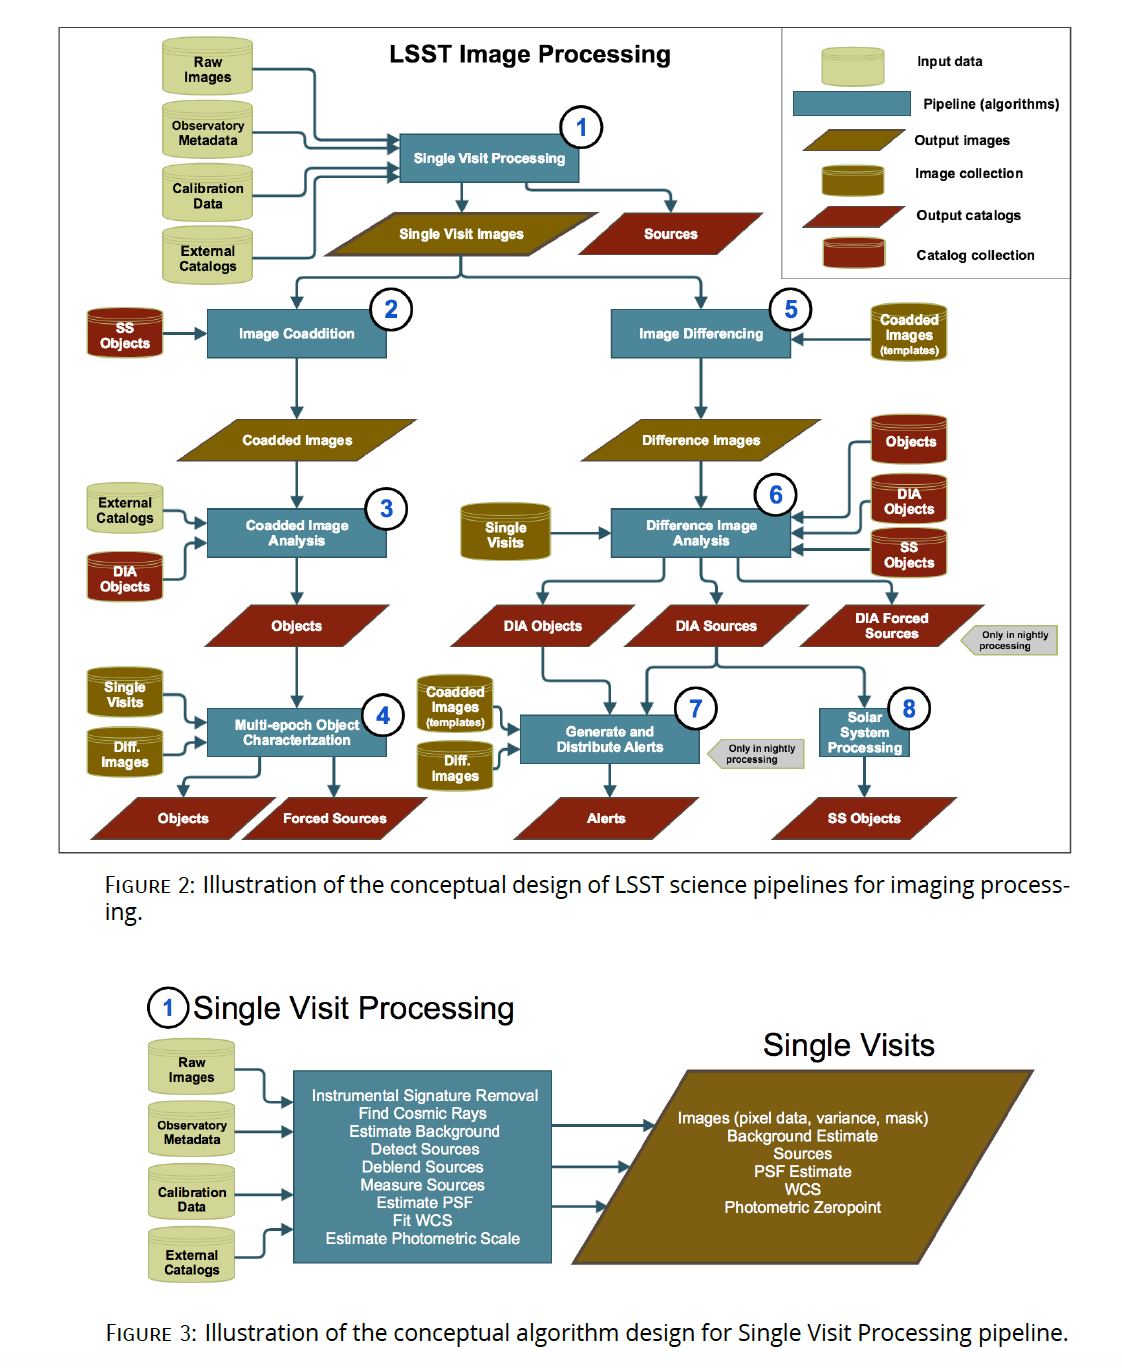
\includegraphics[width=12cm, height=12cm]{figs/dm/DMpipelines1.png}
\end{frame}

\begin{frame}{Rubin-LSST science pipeline}
\begin{tabular}{cc}
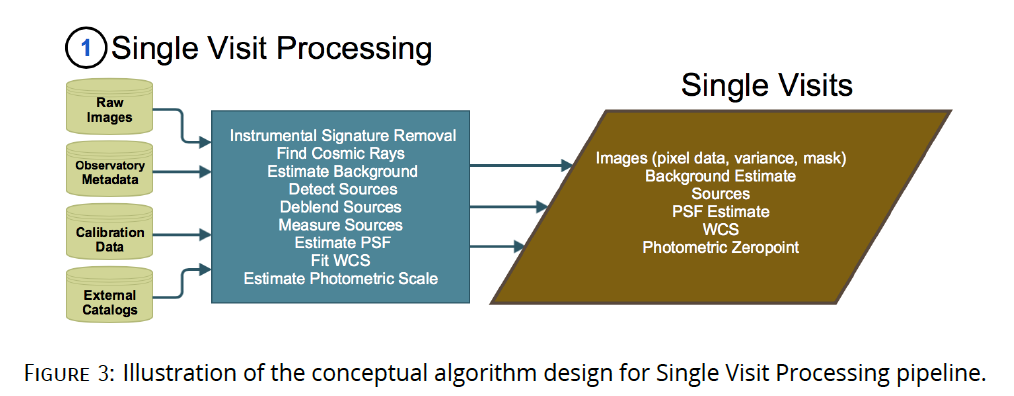
\includegraphics[width=6cm, height=3.5cm]{figs/dm/DMpipelines11.png}
&
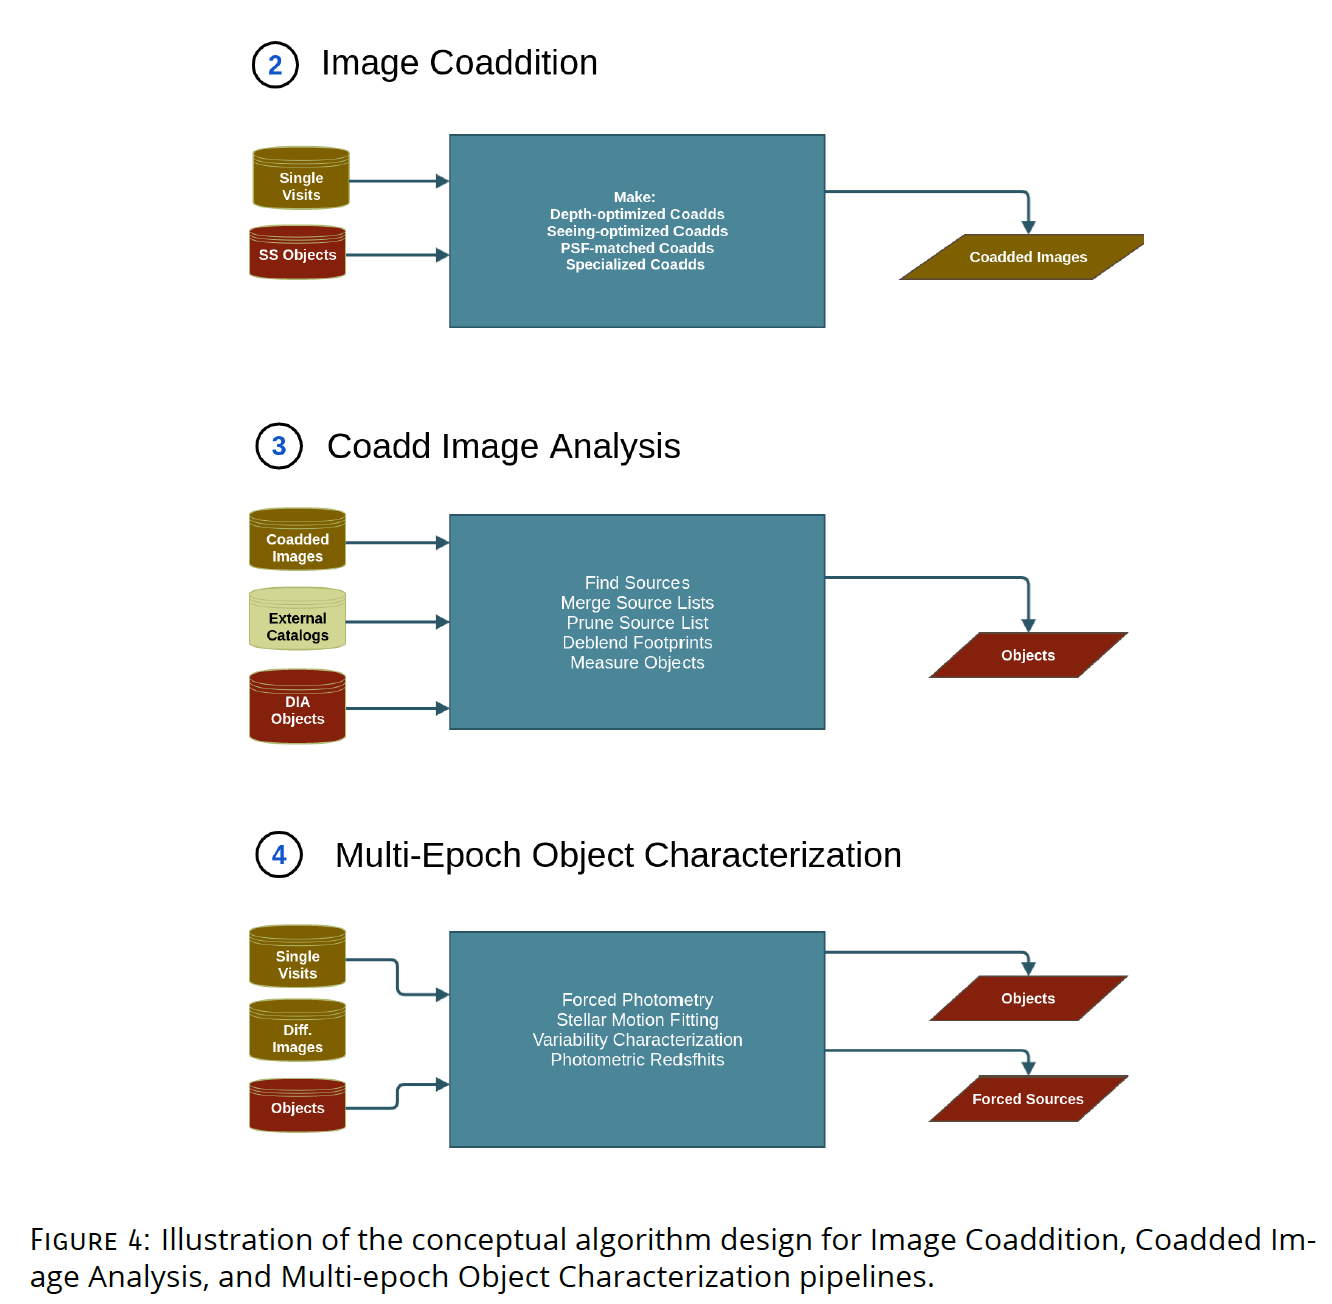
\includegraphics[width=6cm, height=8cm]{figs/dm/DMpipelines2.png}
\end{tabular}
\end{frame}

\begin{frame}{Rubin-LSST calibration plan}
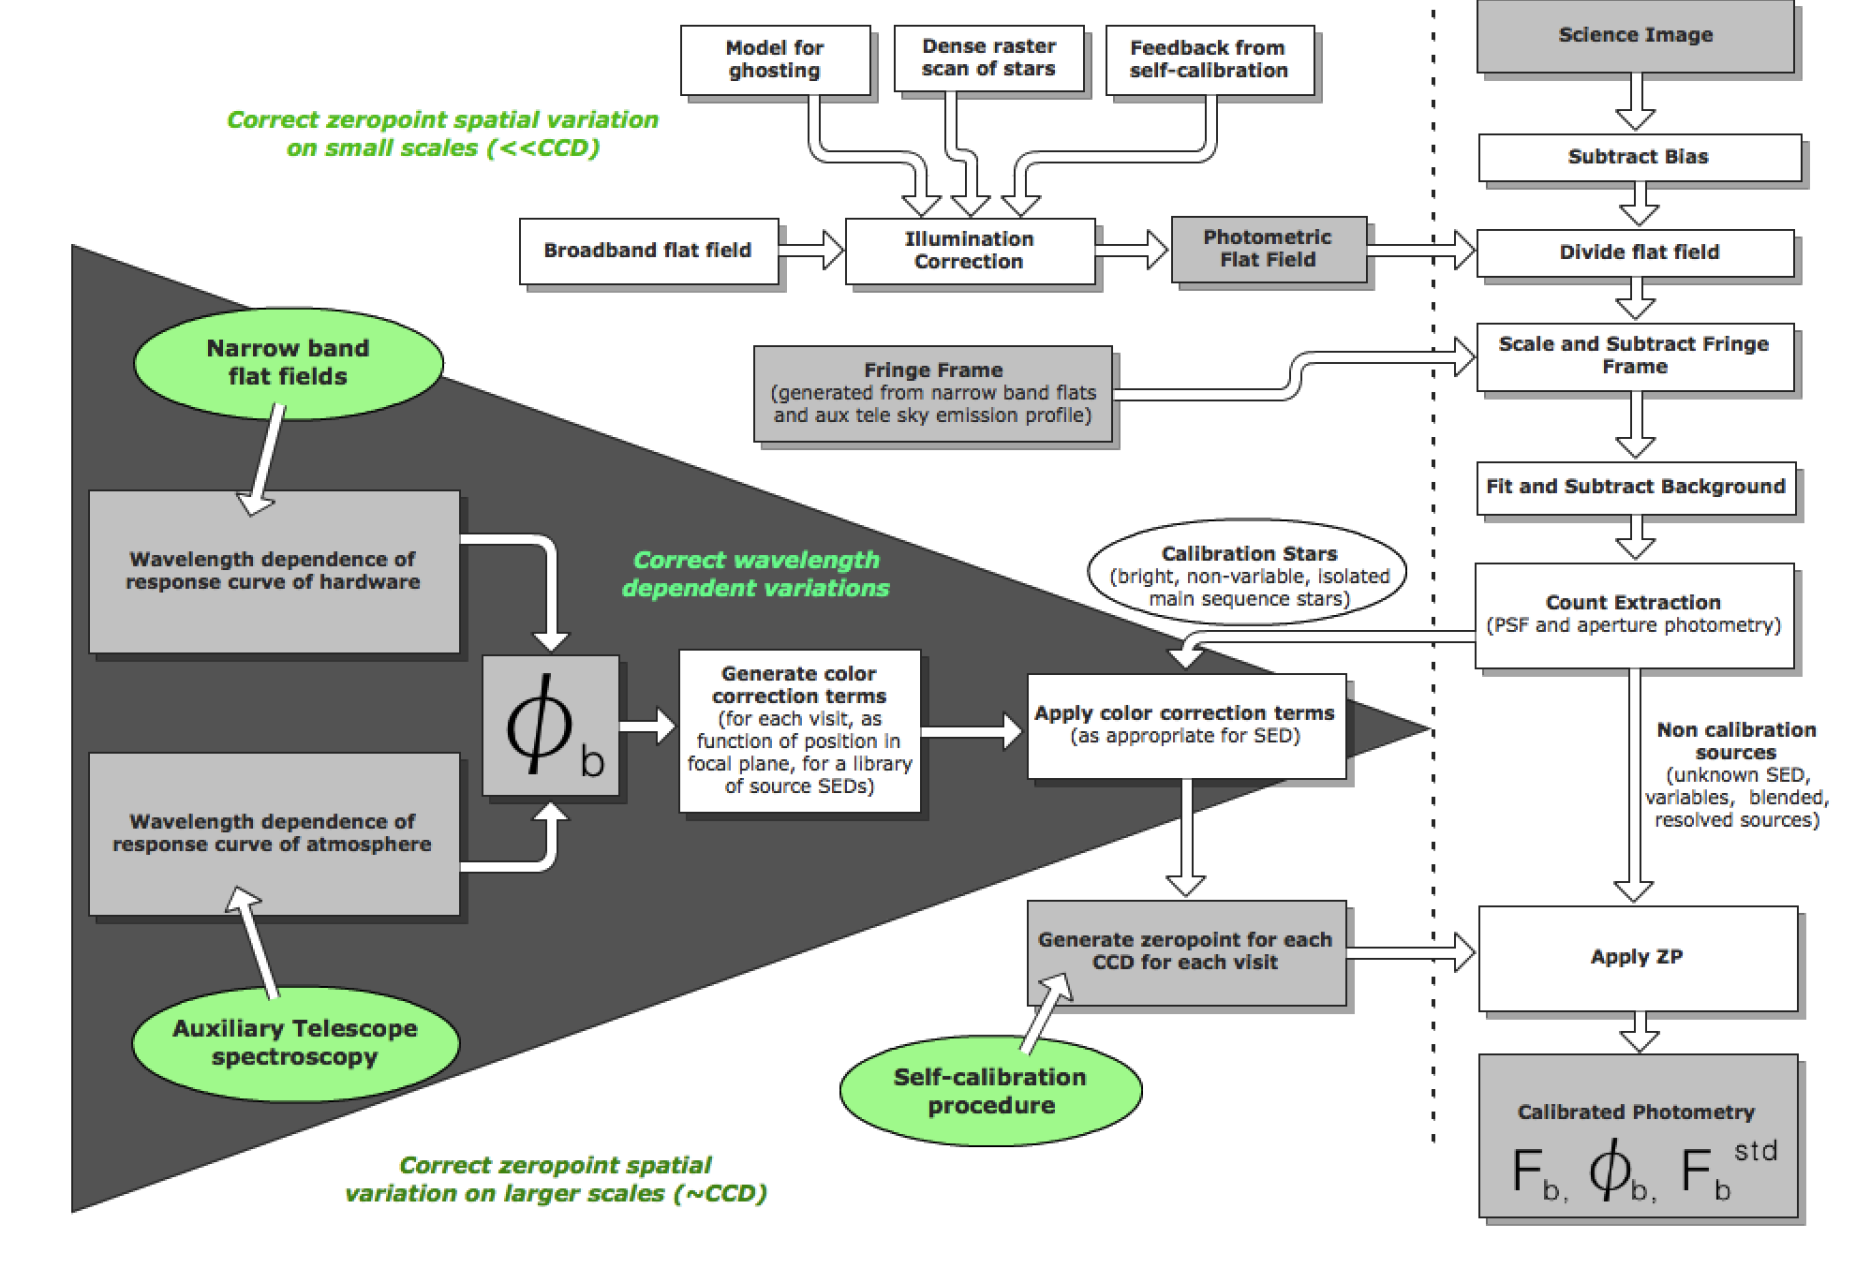
\includegraphics[width=12cm, height=8cm]{figs/calib/LSSTCalibrationPlan.png}
\end{frame}


\section{Simulation of the photometric corrections}

\subsection{Atmospheric simulation and $S_b^{obs}$}
%====================================================================
\begin{frame}{Atmospheric simulation and $S_b^{obs}$}
\begin{tabular}{cc}
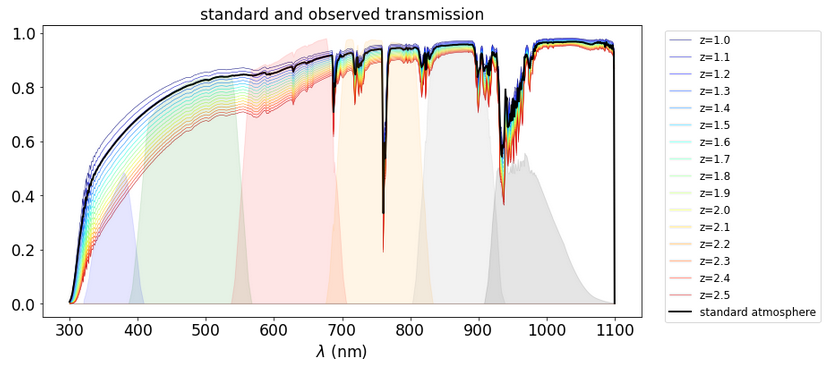
\includegraphics[width=5.9cm, height=3.5cm]{figs/atmsimu/atmsimvsairmass.png} & 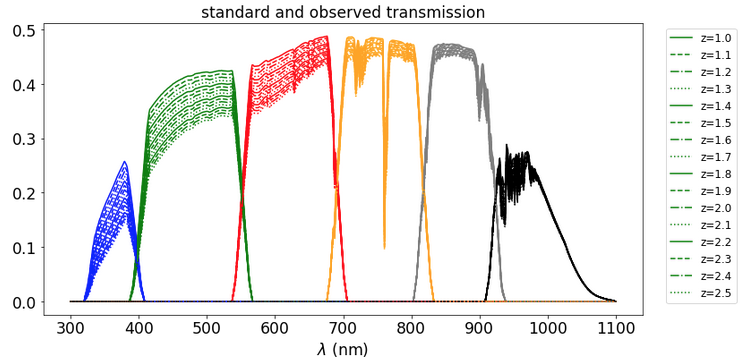
\includegraphics[width=5.9cm, height=3.5cm]{figs/atmsimu/trb_vs_airmass.png} \\
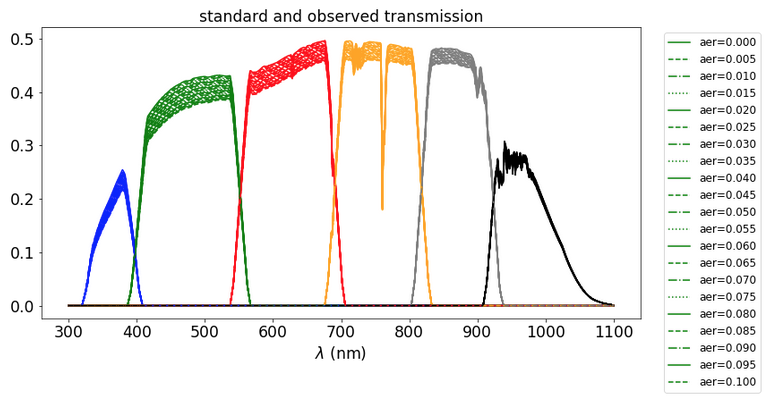
\includegraphics[width=5.9cm, height=3.5cm]{figs/atmsimu/trb_vs_VAOD.png} & 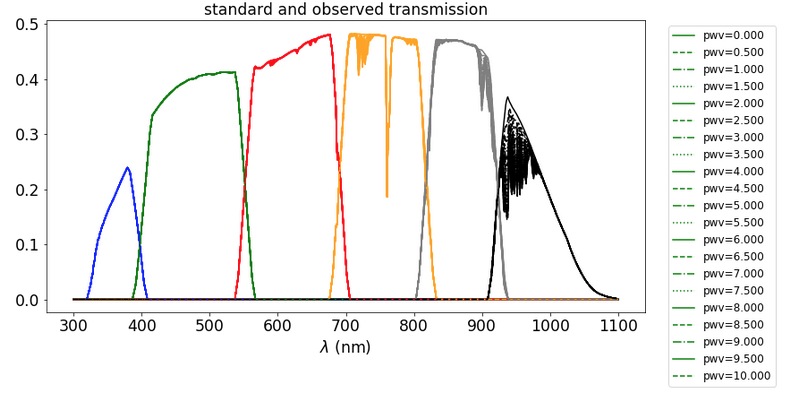
\includegraphics[width=5.9cm, height=3.5cm]{figs/atmsimu/trb_vs_PWV.png}
\end{tabular}
\end{frame}
%====================================================================


\subsection{The zero's order of the photometric correction}
%====================================================================
\begin{frame}{The $0^{th}$ order of the photometric correction}
\begin{alertblock}{vs airmass, relative to the standard transmission}
\begin{equation}
\mathbb{I}^{obs}_{0}(b,z) - \mathbb{I}^{std}_{0}(b,z_{std})
\end{equation}
\end{alertblock}
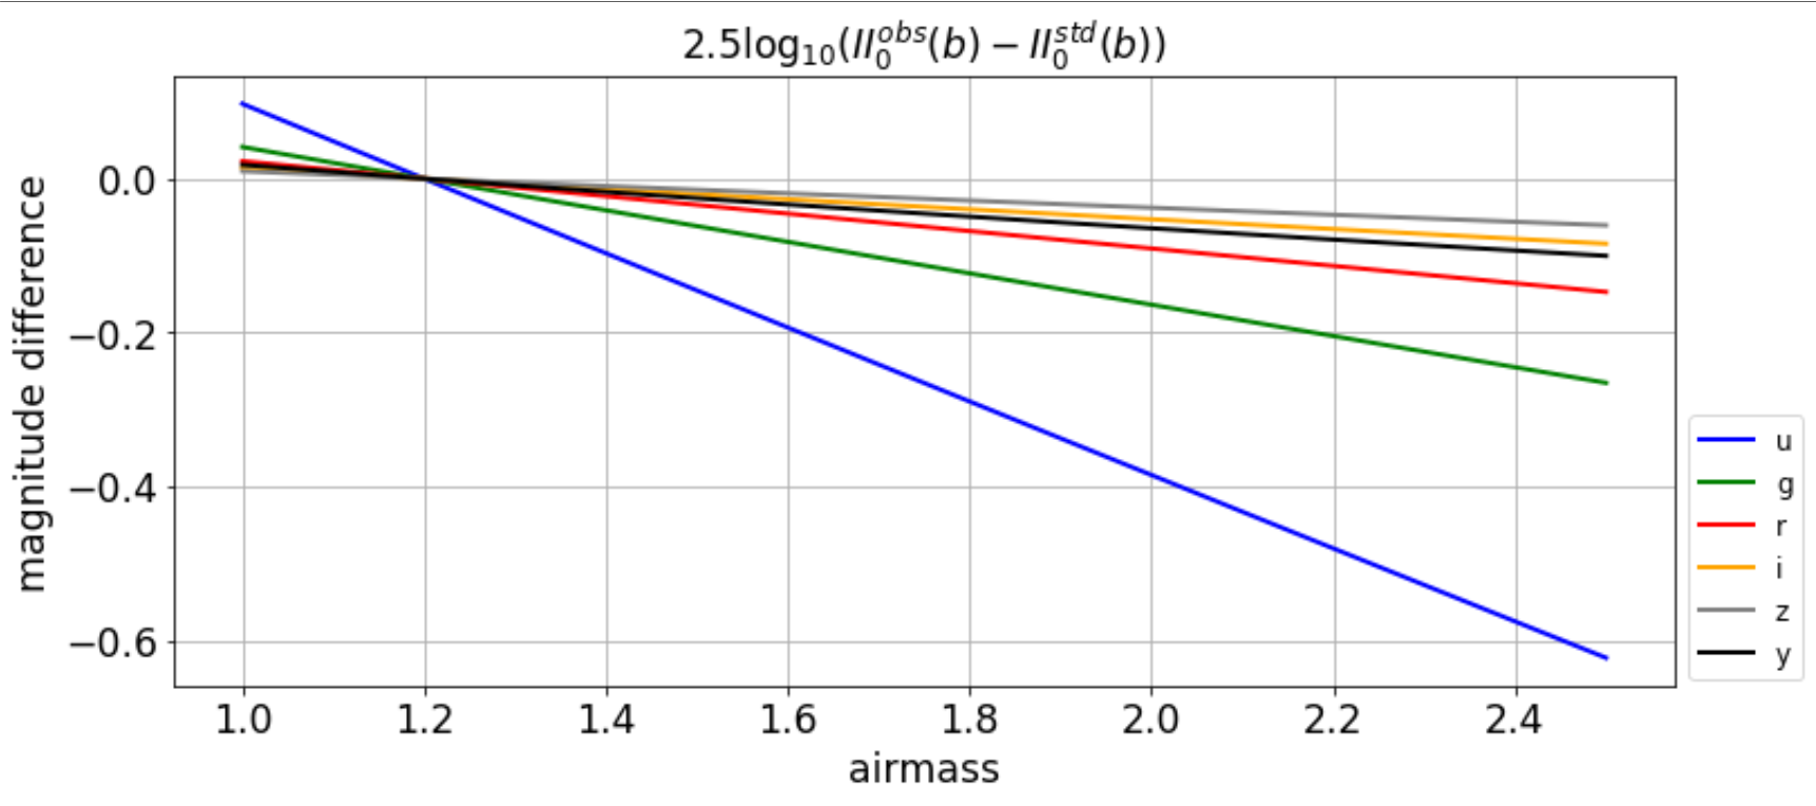
\includegraphics[width=10cm, height=5cm]{figs/Integrals_II/Integrals_II0_vs_airmass.png}
\end{frame}
%====================================================================


%====================================================================
\begin{frame}{The $0^{th}$ order of the photometric correction}
\begin{alertblock}{vs aeorols or PWV, relative to the standard transmission}
\begin{equation}
\mathbb{I}^{obs}_{0}(b,z_{std}) - \mathbb{I}^{std}_{0}(b,z_{std})
\end{equation}
\end{alertblock}
\begin{tabular}{cc}
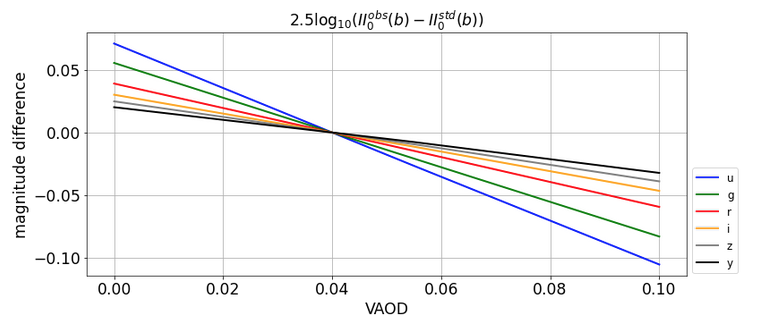
\includegraphics[width=5.9cm, height=4cm]{figs/Integrals_II/Integrals_II0_vs_VAOD.png} & 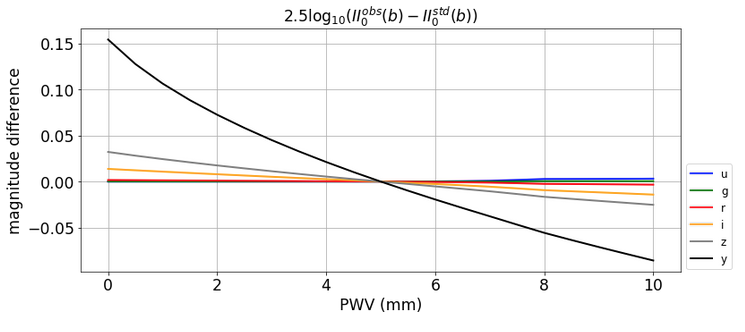
\includegraphics[width=5.9cm, height=4cm]{figs/Integrals_II/Integrals_II0_vs_PWV.png}
\end{tabular}
\end{frame}
%====================================================================

\subsection{The 1st and 2nd orders Integral differences}
%====================================================================
\begin{frame}{The $1^{st}$\&$2^{nd}$ orders Integral differences}

\begin{tabular}{cc}
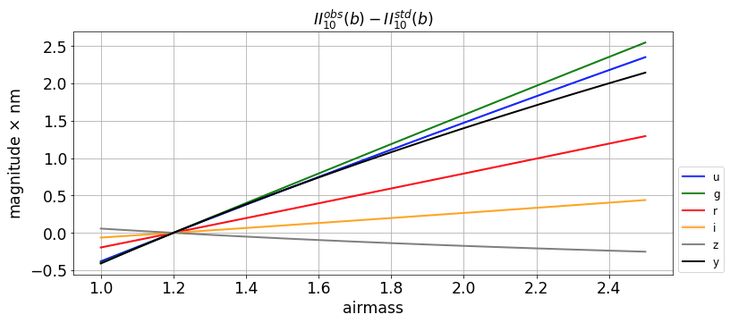
\includegraphics[width=5.9cm, height=4cm]{figs/Integrals_II/Integrals_II10_vs_airmass.png} & 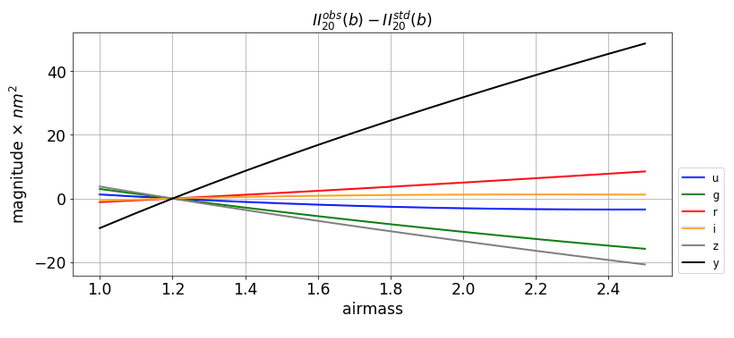
\includegraphics[width=5.9cm, height=4cm]{figs/Integrals_II/Integrals_II20_vs_airmass.png}
\end{tabular}
\end{frame}
%====================================================================


%==========================================================================================================================
\begin{frame}
\begin{center}
{\usebeamerfont{frametitle}

\LARGE \alert{End of part 1}}

\end{center}

\end{frame}
%==========================================================================================================================

 
\end{document}


